\chapter[Otimização multiobjetivo]{Otimização multiobjetivo}

A otimização multiobjetivo consiste em selecionar as melhores soluções de acordo com múltiplos critérios ao invés de apenas um. Por exemplo, ao estabelecer um melhor caminho entre duas cidades pode-se não estar interessado apenas na menor distância, mas também no tráfego, segurança das vias, quantidade de pedágios, etc. A otimização de apenas um objetivo é simples, para que uma solução seja considerada melhor que a outra, basta que ela tenha uma melhor avaliação. Por outro lado, quando se trabalha com mais de uma função de otimização, é preciso usar o conceito de dominância de Pareto.

A dominância de Pareto diz que uma solução $A$ é melhor que uma solução $B$, ou $A$ domina $B$ ($A \prec B$), se, e somente se:

\begin{itemize}  
	\item $A$ é melhor avaliado que $B$ em pelo menos um dos objetivos;
	\item $A$ não tem avaliação pior que $B$ em nenhum dos objetivos.
\end{itemize}

Considerando um problema de minimização e $F$ como o conjunto de funções objetivo, tem-se, matematicamente:

\[A \prec B \Leftrightarrow (\forall(f \in F) f(A) \leq f(B)) \land (\exists (f \in F) f(A) < f(B))\]

Em problemas de otimização multiobjetivo, o interesse está em encontrar o conjunto de todas as soluções que não são dominadas por nenhuma outra, ou seja, a fronteira de Pareto. Graficamente, a fronteira de Pareto representa a linha formada pelas soluções não-dominadas existentes para o problema. Na figura \ref{fig_pareto} apresenta-se um exemplo de uma fronteira de Pareto para um problema de minimização com dois objetivos ($F1$ e $F2$), a fronteira de Pareto está representada em vermelho. Observe que nenhum círculo vermelho possui ambos F1 e F2 menores que alguma outra solução em vermelho, ou seja, são não-dominadas. Em contra-partida, toda solução acima da fronteira, em cinza, é dominada, pois existe alguma solução em vermelho que possui ambos valores de F1 e F2 menores. Caso o problema em questão fosse de maximização, a fronteira de Pareto estaria acima de qualquer solução não-dominada ao invés de abaixo.

\begin{figure}
	\label{fig_pareto}
	\caption{Fronteira de Pareto}
	\centering
	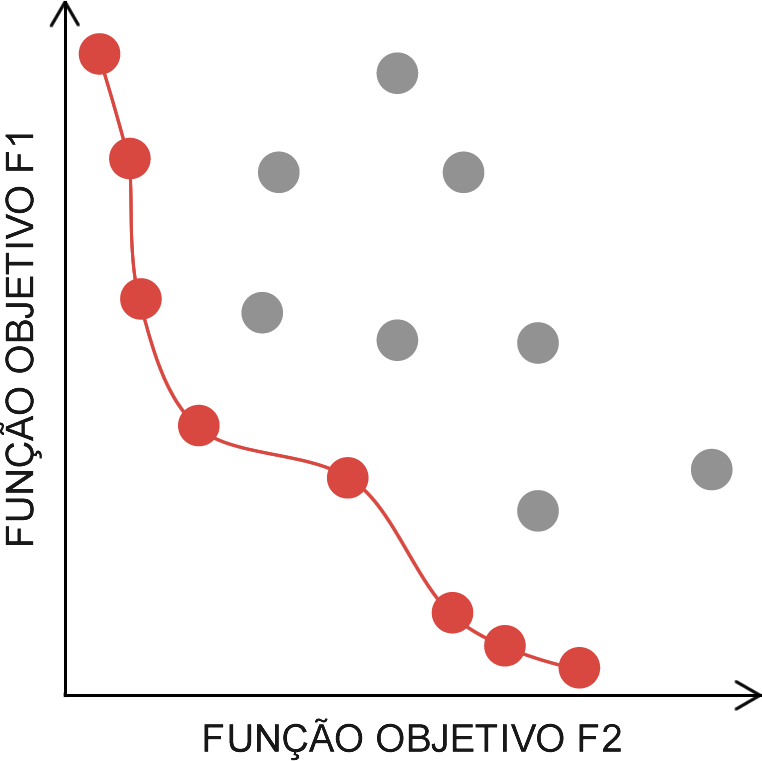
\includegraphics[width=0.4\textwidth]{cap_otimizacao-multi/figs/pareto}
\end{figure}

Não existe limite para o número de funções objetivo em um problema de otimização, mas quanto maior a quantidade de objetivos, mais complexa é a busca. Os algoritmos clássicos de otimização multiobjetivo \ac{NSGA-II} e \ac{SPEA2} lidam bem com até três objetivos, mas a partir de quatro critérios de otimização, ambos os métodos sofrem para encontrar soluções relevantes. Desta forma, criou-se a classificação ``\textit{many-objective}''. Problemas \textit{many-objectives} (4 ou mais objetivos) apresentam diversas novas dificuldades e precisam de novas técnicas para que sejam resolvidos eficientemente. Como observado por Deb em \cite{Deb2014}, os problemas trazidos pelo alto número de objetivos são:

\begin{enumerate}  
	\item Grande parte da população é não dominada: a maioria dos algoritmos multiobjetivos classifica a população de acordo com a dominação de Pareto. Se existem muitas funções objetivo, se torna muito comum que uma solução seja melhor que outra em pelo menos uma das funções. Desta forma, a maior parte das soluções se torna não-dominada, o que impede os algoritmos de evoluírem a população, já que todos os indivíduos são considerados igualmente bons.
	\item Avaliar a diversidade da população se torna computacionalmente caro: afim de garantir uma boa diversidade populacional, alguns algoritmos medem alguma espécie de distância entre as soluções e removem as que são consideradas mais similares. A maior dimensionalidade traz consequentemente um maior impacto no cálculo da proximidade entre os indivíduos. 
	\item \textit{Crossover} ineficiente: a alta dimensionalidade do espaço de busca faz com que os indivíduos na população sejam muito distante uns dos outros e, normalmente, o cruzamento entre duas soluções muito diferentes resultam num filho muito distante dos pais, o que prejudica a convergência da busca. Portanto, pode ser necessário redefinir os operadores de recombinação afim de restringir as possibilidades de pareamento.
	\item População demasiadamente grande: quanto maior o número de objetivos, maior o número de soluções na fronteira de Pareto, portanto, para se obter bons resultados, é necessário que se manipule grandes populações de indivíduos, o que é computacionalmente caro e dificulta o trabalho do usuário que deverá escolher uma única solução ao final do processo.
	\item Métricas de avaliação se tornam difíceis de se calcular: a avaliação das soluções está diretamente relacionada ao número de objetivos, quanto maior ele for, maior será o esforço computacional necessário. A complexidade do hiper-volume, por exemplo, cresce exponencialmente com o número de objetivos.
	\item Dificuldade de visualização: é fácil representar graficamente as soluções e a fronteira de Pareto em problemas de até três objetivos. Com 4 funções em diante, se torna difícil tal visualização.
\end{enumerate}

A maior parte dos algoritmos many-objectives (todos mencionados neste trabalho) lidam apenas com os quatro primeiros problemas. As duas últimas não são responsabilidade dos algoritmos de otimização em sí.

\section{Algoritmos Multiobjetivo}

\subsection{Non-dominated Sorting Genetic Algorithm II (NSGA-II)}
O NSGA-II \cite{Deb2002} é o algoritmo evolutivo multiobjetivo (AEMO) mais frequente na literatura. A atribuição de aptidão (\textit{fitness}) se dá pela classificação da população em rankings de dominância (fronteiras), de forma que o primeiro contenha todas as soluções não dominadas, o segundo todos os indivíduos não-dominados excluindo a primeira fronteira, e assim por diante. Quanto melhor o \textit{ranking} de uma solução, melhor sua aptidão e  maior sua chance de sobreviver para a próxima geração. Várias soluções, pertencem à mesma fronteira, a fim de diferenciá-las utiliza-se um cálculo de distância (\textit{crowding distance}), o qual confere melhor avaliação às soluções mais diferenciadas umas das outras, garantindo assim a diversidade da população.

O processo do NSGA-II é semelhante ao do algoritmo genético comum, com diferença no cálculo de aptidão, que é feito por \textit{ranks}, e no cálculo de distâncias, que é inexistente na proposta original do AG. O primeiro passo continua sendo a geração aleatória dos indivíduos, em seguida classifica-se a população em \textit{ranks} de dominância e inicia-se o laço principal, o qual termina assim que a condição de parada é atingida. O laço principal do NSGA-II é dado pelo pseudo-código do algoritmo \ref{alg_nsgaii}.

\begin{algorithm}
	\caption{Laço principal do NSGA-II}
	\label{alg_nsgaii}
	\begin{algorithmic}[1]
		\While {número máximo de gerações não for atingido}
		\State selecione os pares de pais para o crossover
		\State efetue o cruzamento para cada par de pais, gerando os filhos
		\State combine a população de pais com a população de filhos
		\State classifique todas as soluções em fronteiras (\textit{ranks}) de dominância 
		\State calcule a \textit{crowding distance} para cada uma das soluções
		\State aplique a seleção natural sobre a totalidade da população, preservando os indivíduos de melhor \textit{rank} e, em segundo lugar, \textit{crowding distance}.
		\EndWhile
	\end{algorithmic}
\end{algorithm}

A seleção de pais utiliza torneio simples para o sorteio, ou seja, dois elementos da população são escolhidos de forma aleatória, o indivíduo com melhor avaliação é selecionado como um dos pais, sorteia-se mais dois indivíduos, e o melhor dentre eles se torna o segundo pai.

Na linha 2 do pseudo-código, através dos pares de pais, gera-se os filhos com o \textit{crossover} e a mutação. Após a geração dos filhos, a população corrente e o conjunto de filhos são concatenados (linha 3) e submetidos à classificação em \textit{ranks} de dominância (linha 4).

A classificação em \textit{ranks} de dominância recebe um conjunto de soluções e verifica quais dentre elas não são dominadas. O conjunto de soluções não-dominadas forma o primeiro \textit{rank} de dominância. Do conjunto restante (excluindo o primeiro \textit{rank}), retira-se as soluções não dominadas para formar o segundo \textit{rank}. Esse processo se repete até que todos os indivíduos tenham sido classificados.

Após toda a população ter sido classificada em \textit{ranks}, antes de selecionar os indivíduos que vão compor a população na próxima iteração, deve-se calcular a distância de aglomeração (\textit{crowding distance}) para cada indivíduo em cada \textit{rank} de dominância. O cálculo de distância, para cada objetivo, ordena o conjunto de soluções e faz uma relação entre as distâncias de cada indivíduo para os vizinhos imediatamente anterior e posterior. Soma-se as distâncias obtidas em cada objetivo para cada solução e define-se aquelas com maior valor de distância como as mais diferentes entre sí.

Com toda a população classificada em \textit{ranks} (ou fronteiras) e todas as distâncias calculadas, basta formar a nova população com os melhores indivíduos. Para isso, analisa-se fronteira a fronteira, da melhor para a pior, até que o tamanho máximo da população seja atingido. Para cada fronteira aplica-se o seguinte processo de decisão:

\begin{itemize}  
	\item Se $tamanho(rank) + tamanho(nova_população) < tam_max_pop$: adiciona-se todos os membros do \textit{rank} à nova população.
	\item Caso contrário, se $tamanho(nova_população) < tam_max_pop$: adiciona-se à nova população os $tam_max_pop - tamanho(nova_população)$ elementos do \textit{rank} com os maiores valores de distância. Termine o processo, a nova população está formada.
	\item Caso contrário, termine o processo, a nova população está formada.
\end{itemize}

Desta forma, ao final do algoritmo obtém-se a fronteira de Pareto aproximada na primeira fronteira da população gerada na última iteração do algoritmo.

\subsection{Strength Pareto evolutionary algorithm 2 (SPEA2)}

O SPEA2 \cite{Zitzler2002} é um AEMO que calcula, para cada membro da população, sua força (\textit{strength}) e densidade. A força de uma solução é dada pelo número de indivíduos que ela domina, enquanto a densidade é uma medida de distância para os vizinhos mais próximos, quanto maior a densidade mais próximo o indivíduo está das demais soluções. A aptidão (\textit{fitness}) de uma solução é definida por sua densidade mais a soma das forças de todo indivíduo que a domina. As principais diferenças entre o SPEA2 e um AG comum estão no cálculo de aptidão e na utilização de uma população extra: o arquivo.

O arquivo é responsável por guardar as melhores soluções já encontradas até o momento, funciona como uma espécie de elitismo. Os pais, no cruzamento, são sempre escolhidos do arquivo e os filhos substituem 100\% da população corrente. A cada iteração, os melhores indivíduos entre a população e o arquivo compõe o arquivo da geração seguinte. A quantidade de indivíduos no repositório de soluções não-dominadas é limitada e, portanto, quando se excede o tamanho máximo, deve-se executar um processo de truncamento.

O processo de truncamento do arquivo ocorre na seleção natural, a última função executada na iteração do laço principal de um AG. A seleção no SPEA2 se dá pelo cálculo do arquivo da próxima geração: ambas as populações da iteração corrente (população e arquivo) são submetidas à seleção, extrai-se do conjunto total de soluções aquelas que não são dominadas por nenhuma outra e com esse subconjunto ($n_d$) constrói-se o novo arquivo através do seguinte processo de decisão:

\begin{itemize}  
	\item Se $tamanho(n_d) = capacidade\_arquivo$, o novo arquivo é formado por $n_d$;
	\item Caso contrário, se $tamanho(n_d) < capacidade\_arquivo$, o novo arquivo é formado pela união de $n_d$ com os $capacidade\_arquivo - tamanho(n_d)$ indivíduos restantes com melhor aptidão;
	\item Caso contrário, se $tamanho(n_d) > capacidade\_arquivo$, o novo arquivo é formado por $n_d$ e deve-se truncá-lo em $tamanho(n_d) - capacidade\_arquivo$ passos, onde em cada passo elimina-se o indivíduo com menor variabilidade genética em relação aos demais.
\end{itemize}

Os indivíduos mais aptos no SPEA2 são aqueles dominados pela menor quantidade de soluções e que possuem maior variabilidade genética. O algoritmo calcula a aptidão em três etapas: cálculo de força (\textit{strength}), do \textit{raw fitness} e da densidade.

A força de um indivíduo $i$ ($s(i)$) é o número de soluções que ele domina, ou seja, considerando $A$ o arquivo e $P$ a população:

\[ s(i) = |j|: j \in P \cup A \land i \prec j \]

Tendo calculado a força de cada indivíduo, parte-se para o \textit{raw fitness}. O \textit{raw fitness} de um indivíduo $i$ ($r(i)$) é dado pela soma das forças de cada elemento que o domina. Veja a fórmula a seguir:

\[ r(i) = \sum_{j \in A \cup P | j \prec i} s(j) \]

Observe que, caso o indivíduo seja não-dominado, seu \textit{raw fitness} será o menor possível: zero. Após determinar o \textit{raw fitness}, para finalizar o cálculo de aptidão deve-se descobrir a densidade de cada indivíduo ($d(i)$). A densidade é computada de acordo com a distância da solução para seus vizinhos e é dada pela seguinte fórmula:

\[ d(i) = \frac{1}{\sigma_i^k + 2} \]

Na fórmula acima, $\sigma_i^k$ é a k-ésima menor distância entre o indivíduo $i$ e o restante da população. k é a raiz quadrada do tamanho do conjunto de soluções em avaliação, i.e. $k = \sqrt{|P \cup A|}$. O valor de $d(i)$ sempre está no intervalo (0,1). Referencia-se o leitor ao artigo original do SPEA2 \cite{Zitzler2002} para mais detalhes sobre o cálculo de densidade.

Finalmente, a aptidão do indivíduo ($f(i)$) é dada pela soma do \textit{raw fitness} e a densidade: $f(i) = r(i) + d(i)$. Note que, se a solução $i$ é não-dominada, $f(i) < 1$. isso acontece, pois $d(i) < 1$ para qualquer solução e quando $i$ é não-dominada, $r(i) = 0$.

O laço principal do SPEA2 é explicitado no pseudo-código \ref{alg_spea2} e como resposta para o problema, retorna-se o arquivo da última geração computada. Espera-se que, após as diversas iterações, o algoritmo tenha conseguido uma boa aproximação da fronteira de Pareto.

\begin{algorithm}
	\caption{Laço principal do SPEA2}
	\label{alg_spea2}
	\begin{algorithmic}[1]
		\While {número máximo de gerações não for atingido}
		\State a partir do arquivo, selecione os pares de pais para o crossover
		\State efetue o cruzamento para cada par de pais, gerando os filhos
		\State substitua a população corrente pelos filhos
		\State calcule o fitness de todos indivíduos no arquivo e na população
		\State aplique a seleção natural e trunque o arquivo, caso necessário
		\EndWhile
	\end{algorithmic}
\end{algorithm}

\section{Algoritmos Many-objectives}

\subsection{Multiobjective evolutionary algorithm based on decomposition (MOEA/D)}
\label{section_moead}

O MOEA/D \cite{Zhang2007} é um algoritmo que avalia os objetivos através de uma função escalarizadora, se baseando na dominância de Pareto apenas para atualizar o conjunto de soluções não dominadas geradas em cada iteração (arquivo). No MOEA/D, um problema multiobjetivo é decomposto em múltiplos problemas mono-objetivos chamados de células. Cada célula é definida por um vetor de pesos gerado aleatoriamente e representa um indivíduo, ou seja, o número de células é igual ao tamanho da população. Além dos pesos, a célula, ou indivíduo, é composta de uma solução e uma vizinhança. A vizinhança é formada pelos $k$ indivíduos mais próximos de acordo com o vetor de pesos, onde $k$ é um parâmetro do algoritmo que representa o tamanho das vizinhanças. A aptidão (\textit{fitness}) de uma solução é calculada de acordo com sua avaliação em cada objetivo, a função escalarizadora, e o vetor de pesos da célula. Em toda geração, uma nova solução é gerada para cada célula, onde a vizinhança é levada em consideração para a escolha dos pais e seleção natural.

O primeiro passo do MOEA/D é gerar a estrutura de células e vizinhanças, para isso, sorteia-se os vetores de pesos (a soma de cada vetor deve ser igual a um) e para cada um deles, calcula-se os $k$ vetores mais próximos (vizinhança). Essa estrutura é imutável e é utilizada no decorrer de todo o algoritmo. A geração dos vetores de pesos pode ser tanto aleatória quanto seguir uma distribuição pré-definida. Antes de começar o laço principal, gera-se aleatoriamente uma solução para cada célula e calcula-se as aptidões. 

Uma parte fundamental do MOEA/D é a escolha da função escalarizadora, ela é a principal responsável pelo cálculo de aptidão. Em todos experimentos realizados neste trabalho, foi utilizada a soma ponderada, mas outras estratégia como \textit{Penalty-Based Boundary Intersection} e Tchebycheff também podem ser utilizadas \cite{Zhang2007}. A aptidão de uma solução é calculada através da função escalarizadora e do vetor de pesos, por exemplo, se os valores $[2, 9, 5]$ representam a solução $s$ no espaço de objetivos, $[0.3, 0.2, 0.5]$ é o vetor de pesos da célula $c$, e a soma ponderada é a função escalarizadora, então a aptidão de $s$ em $c$ é dada por $2 * 0.3 + 9 * 0.2 + 5 * 0.5 = 4.9$.

No laço principal do MOEA/D, seleciona-se os pais e gera-se os filhos. Para cada célula $c_i$, dois pais são selecionados aleatoriamente em sua vizinhança. Sempre que um filho é gerado, o processo de seleção é realizado logo em seguida. A aptidão do filho é calculada para cada uma das células na vizinhança de $c_i$, substituindo a solução anterior de uma célula caso seu fitness seja melhor. Após o processo de geração de filhos e seleção, atualiza-se o arquivo com as novas soluções não-dominadas.

\subsection{Non-dominated Sorting Genetic Algorithm III (NSGA-III)}

O NSGA-III \cite{Deb2014} é uma extensão do NSGA-II que permite o \textit{framework} funcionar melhor para mais de três objetivos. Ele se diferencia do original apenas na fase de seleção, onde ao invés de usar a distância de aglomeração para diferenciar soluções em uma mesma fronteira, utiliza um método de clusterização, onde os indivíduos são divididos em nichos de acordo com suas similaridades. O NSGA-III é caracterizado pelo processo de atribuição de nicho chamado de classificação não-dominada baseada em pontos de referência. Sua ideia é traçar uma figura geométrica de uma dimensão a menos que o número de objetivos nos pontos extremos da primeira fronteira. Um número pré-definido de pontos de referência equidistantes é distribuído sobre a figura e passa a representar cada um, um nicho. Para classificar uma solução, define-se como nicho o ponto de referência mais próximo. Ao final, toma-se como sobreviventes os pontos nas regiões menos lotadas do espaço de busca. Para mais detalhes sobre o processo de clusterização, referencia-se o leitor ao artigo original [NSGA-III].

\subsection{SPEA2 with Shift-Based Density Estimation (SPEA2-SDE)}

O SPEA2-SDE \cite{Spea2SDE} é uma pequena alteração no algoritmo SPEA2 que o permite trabalhar com 4 ou mais objetivos de forma muito mais eficiente. A única alteração está no cálculo de distância entre duas soluções. Suponha que $s_1$ e $s_2$ sejam dois indivíduos na população e que seus valores no espaço de objetivo sejam, respectivamente, $[5, 10, 351, 7, 15]$ e $[6, 8, 15, 9, 14]$. No SPEA2, a distância entre $s_1$ e $s_2$ é dada pela distância euclidiana dos dois vetores, ou seja, $distancia(s_1, s_2) = \sqrt{(5-6)^2 + (10-8)^2 + (351-15)^2 + (7-9)^2 + (15-14)^2} = 336,0148$. As duas soluções são, na verdade bem próximas, pois só estão distantes em uma das 5 coordenadas, mas o cálculo de distância do SPEA2 não reflete isso, o que é prejudicial em problemas com muitos objetivos. A fim de resolver esse problema, Miqing Li et al. introduziram o cálculo de distância \ac{SDE}, que nada mais faz do que transladar a coordenada mais distante do segundo ponto para o mesmo valor no primeiro ponto, isto é, antes de calcular a distância euclidiana, identifica-se a coordenada que exibe maior diferença entre os dois pontos, no caso dos exemplos $s_1$ e $s_2$, a terceira coordenada é a que possui esse comportamento. Em seguida, modifica-se o segundo ponto na coordenada identificada para que seja igual ao primeiro ponto, no exemplo, cria-se $s_2' = [6, 8, 351, 7, 15]$. A distância SDE é então determinada pela distância euclidiana entre o primeiro ponto e o segundo ponto transladado. No exemplo, a distância final vale $distancia(s_1, s_2') = \sqrt{(5-6)^2 + (10-8)^2 + (351-351)^2 + (7-9)^2 + (15-14)^2} = 3,1622$. A distância SDE, em resumo, descarta a coordenada mais distante ao calcular as distâncias, permitindo assim que pontos distantes em apenas uma coordenada ainda sejam considerados próximos. Todo o restante do processo do SPEA2 segue da mesma maneira que o algoritmo original.

\subsection{Algoritmo Evolutivo Multiobjetivo com Muitas Tabelas (AEMMT)}

O AEMMT \cite{Brasil2013}, assim como o MOEA/D, decompõe o problema multiobjetivo em subproblemas menores e para isso utiliza um esquema de tabelas, onde cada tabela representa uma combinação diferente de objetivos. A função que transforma os múltiplos objetivos em um valor escalar é sempre a média e cada tabela mantém os melhores indivíduos considerando a média dos objetivos que representa. A cada geração, duas tabelas são selecionadas para o cruzamento. Dois pais, um de cada tabela, são sorteados aleatoriamente para gerarem um único filho, que será testado em todas as tabelas, entrando naquelas em que representar uma melhor aptidão em relação aos demais indivíduos. Naturalmente, como um único \textit{crossover} é realizado a cada iteração, o AEMMT precisa de mais gerações para efetuar o mesmo número de comparações que os algoritmos citados nas seções anteriores.

A quantidade de tabelas é determinada pelo número de combinações possíveis de objetivos. Para quatro objetivos ($f_1, f_2, f_3, f_4$), por exemplo, como ilustrado na figura \ref{fig_aemmt_tabelas} serão criadas 15 tabelas de combinações mais uma tabela extra, usada para guardar os indivíduos não-dominados.

\begin{figure}
	\label{fig_aemmt_tabelas}
	\caption{Tabelas do AEMMT}
	\centering
	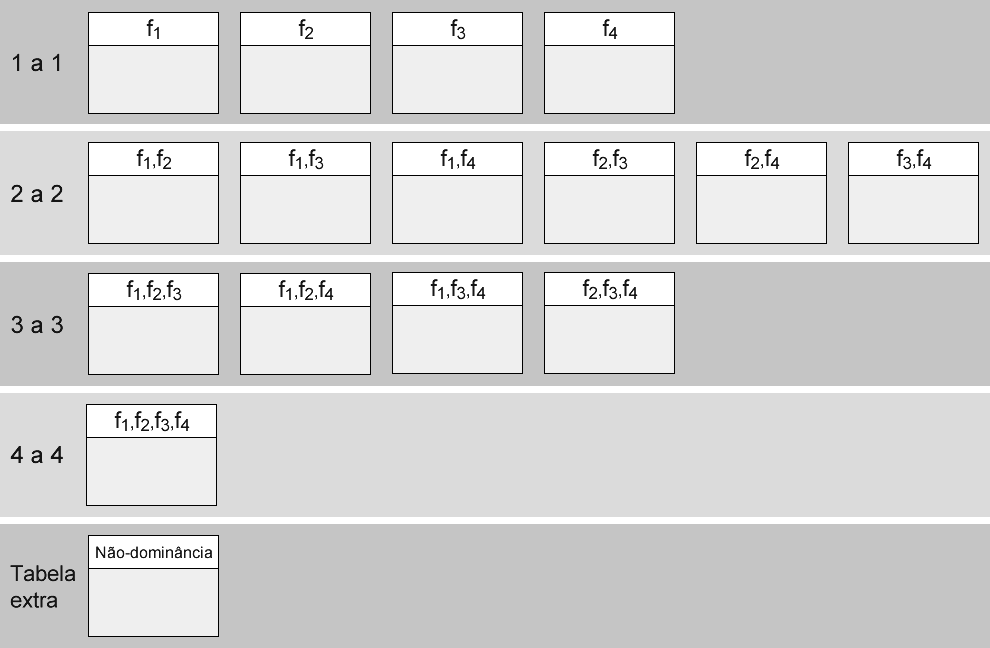
\includegraphics[width=1\textwidth]{cap_otimizacao-multi/figs/aeemt-tabelas}
\end{figure}

Cada tabela possui um limite máximo de indivíduos e no início do algoritmo gera-se soluções aleatórias de forma que todas as tabelas sejam completamente preenchidas. No laço principal, um indivíduo só entra em uma tabela $t$ se for melhor que a pior solução na população de $t$. Com relação a tabela de dominância, sempre que um filho é gerado e não-dominado por nenhum outro indivíduo na tabela, ele é incluído. A restrição no tamanho da tabela de dominância é independente das demais e sempre que o limite for atingido, é feito um truncamento priorizando a permanência das soluções com maior valor de média aritmética entre todos os objetivos.

O primeiro passo do AEMMT é gerar as tabelas e preenchê-las com soluções aleatórias. Em seguida, inicia-se o laço principal, onde em cada iteração são escolhidas duas tabelas via torneio duplo de acordo com suas pontuações. A pontuação tem valor inicial zero e sempre que uma tabela gera um filho que sobrevive para a geração seguinte, sua pontuação é incrementada. As pontuações são zeradas a cada 100 gerações. Considerando as duas tabelas que vencem os torneios, sorteia-se um indivíduo de cada e efetua-se o cruzamento entre os dois. O filho gerado é então comparado tabela à tabela, entrando naquelas em que representar uma melhoria. Após a execução de todas as gerações, dá-se como resultado o conjunto não dominado entre as soluções de todas as tabelas.

\subsection{Algoritmo Evolutivo Multiobjetivo com Múltiplas Dominâncias (AEMMD)}
\label{section_aemmd}

O AEMMD \cite{Lafeta2016}, é uma modificação do AEMMT que, apesar de usar o mesmo processo de divisão do problema multi-objetivo, abandona a ideia de escalarização e volta a utilizar o conceito de dominância dos métodos mais antigos (e.g. NSGA-II e SPEA2). No AEMMD, ao invés de se utilizar a média dos objetivos da tabela para avaliar o indivíduo, lança-se mão da relação de dominância de Pareto, um indivíduo novo $s$ só entra na tabela $t$, se $s$ não for dominado por nenhuma solução em $t$ considerando apenas os objetivos de $t$. Além disso, se $s$ entra em $t$, todas as soluções em $t$ dominadas por $s$ são removidas.

O primeiro passo do AEMMD é gerar o conjunto de tabelas, que é composto por todas as combinações de objetivos possíveis a partir de dois a dois. Combinações de um único objetivo não são criadas, pois o conceito de dominância é válido apenas para a partir de dois valores. Diferentemente do AEMMT, as tabelas não possuem limite de tamanho e podem crescer indefinidamente. Para um problema de quatro objetivos ($f_1, f_2, f_3, f_4$), por exemplo, 11 tabelas seriam geradas, veja a figura \ref{fig_aemmd_tabelas}.

\begin{figure}
	\label{fig_aemmd_tabelas}
	\caption{Tabelas do AEMMD}
	\centering
	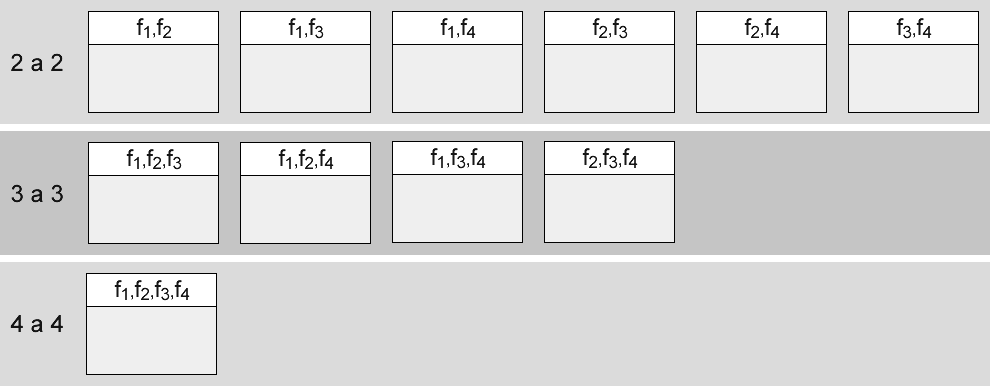
\includegraphics[width=1\textwidth]{cap_otimizacao-multi/figs/aeemd-tabelas}
\end{figure}

Com as tabelas criadas, gera-se um número pré-definido de soluções aleatórias, distribuindo-nas pelas tabelas de acordo com a relação de dominância de Pareto. O próximo passo é o laço principal, onde a cada iteração, através de um torneio duplo, sorteia-se duas tabelas de acordo com suas pontuações. A pontuação das tabelas no AEMMD é diferente do AEMMT, ao invés de conceder um ponto sempre que se gera um indivíduo sobrevivente, pontua-se uma tabela quando ela recebe um indivíduo. Tendo escolhido as duas populações pais, sorteia-se um representante de cada e gera-se um único filho, o qual é comparado tabela à tabela e entra naquelas onde representa uma solução não dominada. Outra diferença em relação ao método original, é que o AEMMD não reinicia as pontuações em momento algum do algoritmo. Espera-se que ao final das gerações, a população da tabela principal, com todos os objetivos, tenha convergido para a fronteira de Pareto. 

\section{Algoritmos \textit{many-objectives} baseados em colônias de formigas}

A maior parte dos métodos de busca multiobjetivo são baseados em algoritmos genéticos, mas uma boa alternativa pouco explorada é a inteligência coletiva, representada por estratégias como as colônias de formigas (ACOs) e enxame de partículas (PSOs). Neste trabalho, devido ao fato de explorar-se dois problemas discretos (problema da mochila multiobjetivo e problema do roteamento multicast), optou-se por utilizar as colônias de formigas, que foram desenvolvidas especialmente para lidar com esse tipo de problema. Como explicado em [secao\_formigas], ao invés de utilizarem os operadores genéticos para gerarem e evoluírem a população, os ACOs lançam mão de um processo de construção de solução baseado em feromônios, o qual decide, a cada passo, uma partícula da solução de acordo seu valor de feromônio e heurística. Dentre os ACOs multiobjetivos propostos na literatura, destacam-se o MOACS, ...

\subsection{Multi-Objective Ant Colony Optimization Algorithm (MOACS)}

O MOACS foi proposto pela primeira vez em \cite{Baran2003} para o problema de roteamento de veículos com janelas de tempo e posteriormente foi aplicado no problema do roteamento multicast \cite{Pinto2005}. A última versão do algoritmo foi proposta em \cite{Riveros2016} e essa é a variação utilizada neste trabalho. O MOACS é uma adaptação do ACO original que torna possível a otimização de múltiplos objetivos utilizando uma única estrutura de feromônios, múltiplas heurísticas e um arquivo de soluções não dominadas. Veja o código do algoritmo \ref{alg_moacs}.

\begin{algorithm}
	\caption{Algoritmo MOACS}
	\label{alg_moacs}
	\begin{algorithmic}[1]
		\State Inicialize a estrutura de feromônios $\tau_{ij}$ com $\tau_0$ /* $\tau_{0}$ é o valor inicial */
		\State Crie um conjunto vazio de soluções não-dominadas $ND$
		\While {Número máximo de iterações não for atingido}
		\For {$i \gets 0$ até $tamanho\_populacao$}
		\State Sorteie valores no intervalo $[0, w_{max}[$ para formar um vetor de pesos $W$ com $|H|$ posições
		\State Construa uma solução de acordo com a tabela de feromônios $\tau_{ij}$, as heurísticas ($H$) e os pesos $W$
		\State Atualize $ND$ com a nova solução
		\EndFor
		\If {$ND$ foi modificado}
		\State Reinicie a estrutura de feromônios fazendo $\tau_{ij} = \tau_0 \forall(i,j)$
		\Else
		\State Atualize a estrutura de feromônios com todas as soluções em $ND$
		\EndIf
		\EndWhile
		\State \Return $ND$
	\end{algorithmic}
\end{algorithm}

O processo de construção da solução depende do problema e, no MOACS, os principais componentes para o processo são:

\begin{itemize}  
	\item Feromônios ($\tau_{ij}$): estrutura que guarda a quantidade de feromônios em cada partícula que pode formar a solução. No caso de problemas em grafos, representa a quantidade da substância em cada uma das arestas;
	\item Heurísticas ($H$): conjunto de funções que estimam a qualidade de uma dada partícula que pode formar a solução. No caso de problemas em grafos, representa os vários pesos em uma aresta. Por exemplo, num grafo que representa uma rede de computadores com informações de custo, distância e tráfego, $H$ poderia ser formado de três funções que recebem uma aresta $(i,j)$ e devolvem, respectivamente, os valores de peso, distância e tráfego na aresta.
	\item Peso máximo de uma heurística ($w_{max}$): representa o valor máximo que o peso de uma heurística pode atingir. Em \cite{Riveros2016}, propõe-se $w_{max} = 3$, de forma que cada função possa ser classificada como 0 (não importante), 1 (importante), 2 (muito importante).
	\item Vetor de pesos ($W$): O vetor de pesos atribui a importância de cada heurística e é gerado aleatoriamente em cada iteração. Cada função de heurística recebe um peso variando no intervalo $[0, w_{max}[$.
\end{itemize}

Ao construir uma solução, utiliza-se o mesmo processo de decisão do ACO original, explicado na seção \ref{section_construcao_solucao}. A única diferença é que as múltiplas heurísticas do MOACS ($H$) deve ser unificada em uma única função $h(x)$, para isso utiliza-se o vetor de pesos $W$ para se aplicar uma média ponderada. Veja a equação a seguir:

\[h(x) = \frac{\sum_{i \gets 0}^{size(H)}\ H_i(x) * W_i}{\sum_{w \in W} w}\]

Em cada época (iteração do laço principal), atualiza-se o arquivo de soluções não dominadas com as novas soluções geradas. Se o arquivo foi atualizado após criar-se todas as soluções, reinicia-se as informações de feromônio, redefinindo todos os valores na estrutura $\tau_{ij}$ para o valor inicial de feromônio $\tau_0$. Caso o arquivo tenha se mantido estável, ou seja, nenhuma das novas soluções seja não-dominada, atualiza-se as quantidades de feromônio na estrutura de acordo com as soluções no arquivo.

Considerando um problema em grafos, para atualizar a estrutura $\tau_{ij}$ com uma solução $s$, faz-se:

\[\tau_{ij} = (1 - \rho) * \tau_{ij} + \rho * \Delta\tau(s) \forall(i,j) \in s\]

Onde:
\begin{itemize} 
	\item $\rho$: coeficiente de evaporação;
	\item $\Delta\tau(s)$: Quantidade de feromônios depositados pela solução $s$.
\end{itemize}

A quantidade de feromônio depositado pela solução $s$ ($\Delta\tau(s)$) é definida por:

\[\Delta\tau(s) = \frac{1}{performance(s)}\]

Na fórmula anterior, $performance(s)$, é dado pela soma dos valores de $s$ no espaço de objetivos. Neste caso, considera-se um problema de minimização, para problemas de maximização, basta inverter a equação. Se os objetivos são reduzir o custo, o tráfego e o delay de uma rede, por exemplo, $performance(s) = custo(s) + trafego(s) + delay(s)$.

Após todas as iterações do laço principal, espera-se obter no arquivo uma boa aproximação da fronteira de Pareto. 

\subsection{Multiobjective evolutionary algorithm based on decomposition and ACO (MOEA/D-ACO)}
O MOEA/D-ACO \cite{Ke2013} é o algoritmo MOEA/D (seção \ref{section_moead}) aplicado ao \textit{framework} de otimização por colônia de formigas (ACO). Os conceitos de células e vizinhanças são reutilizados, enquanto que a reprodução local, inexistente no ACO, é substituída por um processo de construção da solução levemente modificado. Além disso introduz-se um novo conceito de grupos que é utilizado para \textit{clusterizar} as formigas de acordo com seus vetores de peso. Chama-se de formiga neste algoritmo o que era chamado de célula, no MOEA/D.

O primeiro passo do MOEA/D-ACO consiste em gerar os vetores de peso que, assim como no MOEA/D, são \textit{arrays} de valores entre 0 e 1 cujas somas valem 1. A geração pode ser aleatória ou seguir uma distribuição pré-definida. No caso deste trabalho, utilizou-se a distribuição uniforme proposta no artigo original \cite{Ke2013}. Atribui-se cada vetor a uma formiga e cria-se a estrutura de vizinhanças, onde cada formiga é associada a uma vizinhança contendo as $v_size$ formigas mais próximas de acordo com os vetores de peso (incluindo ela mesma). O segundo passo do algoritmo determina os grupos, cada grupo recebe um novo vetor de pesos gerado da mesma maneira que os pesos anteriores. As formigas são então distribuídas entre os grupos de acordo com a proximidade entre seu vetor de pesos e o vetor de pesos do grupo (\textit{clusterização}).

Com respeito às duas principais estruturas de um ACO, heurística e feromônios, cada formiga possui uma função heurística e cada grupo mantem uma estrutura de feromônios. Quando os grupos são criados, cada um recebe uma estrutura de feromônios com o valor máximo de feromônio em cada uma das posições. A formiga, por sua vez, quando criada recebe uma função heurística baseada na combinação de todas as funções heurísticas do problema e no vetor de pesos da própria formiga. O cálculo específico da heurística depende do problema e será visto na seção \ref{section_estrategias_prm_aco} para o PRM e na seção \ref{section_estrategias_pmm_aco} para o PMM.

O laço principal do MOEA/D-ACO consiste em gerar as soluções, atualizar o conjunto de soluções não-dominadas $ND$, distribuir as novas soluções entre as formigas e atualizar as estruturas de feromônios. Primeiramente, para cada grupo $G$, gera-se as soluções para cada formiga $f \in G$. A solução é gerada com base nos feromônios de $G$, na heurística de $f$ e na solução atual de $f$. Tendo gerado todas as soluções para um grupo, atualiza-se o arquivo de soluções não-dominadas $ND$. Para cada nova solução $S$ que entrou no arquivo, modifica-se a estrutura de feromônios $\tau$ de $G$ de acordo com a fórmula a seguir:

\[
\tau(e)= 
\begin{cases}
\rho * \tau(e),& \text{se } e \notin S\\
\rho * \tau(e) + \delta,              & \text{caso contrário}
\end{cases}
\]

Onde $e$ é qualquer aresta (PRM) ou item (PMM) da tabela de feromônios, $\rho$ é a taxa de evaporação, e $\delta$ é dado pelo inverso da soma dos valores da função de escalarização aplicada sobre cada solução não dominada de $G$ em relação ao vetor de pesos de $G$.

Cada formiga armazena duas soluções, a solução atual, que de início é nula, e a nova solução, criada em cada iteração do laço principal. Após passar por todos os grupos e suas formigas gerando as novas soluções e atualizando os feromônios, deve-se decidir a solução atual de cada formiga com base nas novas soluções da vizinhança, o que é feito da seguinte maneira: para cada formiga $f$, analisa-se as novas soluções presentes na vizinhança de $f$; se alguma nova solução $ns$ que ainda não substituiu nenhuma outra possui um \textit{fitness} melhor que o da solução corrente de $f$ ($sc$), substitui-se $sc$ por $ns$. O \textit{fitness} é calculado de acordo com a média pondera dos valores da solução em cada objetivo baseadas no vetor de pesos da formiga em questão. Neste trabalho utilizou-se a soma ponderada como função \textit{escalarizadora}, mas qualquer uma das funções propostas em \cite{Zhang2007} poderia ter sido usada.

O processo de construção da solução depende do problema e é apresentado nas seções \ref{section_estrategias_prm_aco} para o PRM e  \ref{section_estrategias_pmm_aco} para o PMM. Mas, de qualquer forma, independente do problema, o MOEA/D-ACO inclui duas novas características no processo, são elas:

\begin{itemize}
	\item Influência da solução atual: no MOEA/D-ACO, cada formiga mantem uma solução atual que influencia a construção da próxima solução com base em um parâmetro $\delta$. Isso acontece devido à introdução de um novo termo no cálculo de feromônio na construção da solução. Ao calcular a probabilidade de uma partícula $p$ (aresta ou item) de fazer parte da solução, ao invés de considerar $feromonio(p)^\alpha$, considera-se $(\delta * x + feromonio(p))^\alpha$, onde $x = 1$ se $p$ pertence à solução atual e $x = 0$ caso contrário.
	\item Taxa de elitismo: a maioria dos ACO's utilizam uma espécie de roleta para decidir qual partícula fará parte da solução, aquelas com maior probabilidade terão maior chance de serem escolhidas, mas não necessariamente serão. Em uma estratégia elitista, não há roleta, a partícula escolhida será aquela que receber o maior valor de probabilidade. No MOEA/D-ACO, utiliza-se uma taxa de elitismo, que estipula a chance de uma partícula ser escolhida por elitismo ao invés de roleta.
\end{itemize}

O laço principal é executado até que uma condição de parada pré-definida seja atingida, normalmente um número máximo de iterações. Espera-se que nesse momento as soluções no conjunto $ND$ tenham convergido para a fronteira de Pareto.

\section{Outros algoritmos multiobjetivos}
Alguns outros algoritmos multiobjetivos não foram analisados neste trabalho, mas por serem relacionados ao tema da pesquisa, aproveita-se esta seção para mencioná-los. \ac{VEGA} \cite{Schaffer1985}, \ac{NSGA} \cite{Srinivas1994} e \ac{SPEA} \cite{Zitzler1999} foram os primeiros algoritmos multiobjetivos a aparecerem na literatura, apesar do NSGA-II e SPEA2 serem os mais conhecidos. Quanto aos problemas \textit{many-objectives}, uma das principais dificuldades encontradas é o excesso de soluções não-dominadas, o que dificulta a identificação de melhores indivíduos e prejudica a convergência. Ao se depararem com esse problema, H. Aguirre e K. Tanaka propuseram um novo conceito, menos rigoroso, de dominância, dando origem ao algoritmo $\epsilon$-MOEA \cite{Aguirre2009}. Enquanto isso, a fim de reclassificar as soluções não dominadas e resolver o mesmo problema, Beume et. al. propuseram a evolução da população de acordo com indicadores de qualidade do conjunto de soluções. No algoritmo que apresentaram em 2011, SMS-EMOA \cite{Beume2007}, os autores usam o hiper-volume para avaliar soluções consideradas igualmente boas pela dominância de Pareto. J. Bader e E. Zitzler, em 2011, utilizaram uma ideia parecida ao proporem o algoritmo Hype \cite{Bader2011}, que também utiliza o hiper-volume como parâmetro para guiar a evolução da população. Em \cite{Ishibuchi2015} Ishibuchi apresenta uma comparação entre os principais métodos de otimização aplicados ao PMM e em \cite{Franca2017}, artigo resultante deste trabalho, estende-se a comparação para métodos mais recentes (como o AEMMT) e um novo problema discreto, o PRM.

Sobre os algoritmos de otimização multiobjetivos baseados em colônias de formigas, em 2004 Alaya et al. aplica o \textit{MIN-MAX Ant System} no problema da mochila com múltiplos objetivos e múltiplas restrições \cite{Alaya2004}. Outras aplicações de ACOs no problema da mochila podem ser encontradas em \cite{changdar2013,Ke2010,Fingler2014,kong2008,Fidanova2003}. Souza e Pozo propõe o algoritmo MOEA/D-BACO que aplica uma variação do MOEA/D-ACO no problema de programação binária quadrática irrestrito (UBQP). Como para o UBQP as estruturas de feromônio crescem de forma exponencial em relação ao tamanho da entrada, torna-se inviável a utilização do ACO original e então os autores propõe a substituição do mesmo pelo BACO no MOEA/D-ACO, criando a modificação MOEA/D-BACO \cite{SouzaPozo2015}.